% Standard LLNCS option keeps the ordinary vector accent (compatible with amsmath).
\PassOptionsToClass{orivec}{llncs}
\documentclass[runningheads]{llncs}
\usepackage[T1]{fontenc}
\usepackage{graphicx}
\usepackage{amsmath,amssymb}
\usepackage{booktabs}
\usepackage{algorithm}
\usepackage{algpseudocode}
\usepackage{url}
\usepackage[hidelinks]{hyperref}
\graphicspath{{figures/}}
\newcommand{\astar}{A\ensuremath{^*}}
\newcommand{\source}[1]{\path{#1}}
% Author and affiliation verified by the author; no additional metadata supplied.
\newcommand{\ReportAuthor}{Nguyen Hoang Thang}
\newcommand{\ReportRunningAuthor}{Nguyen Hoang Thang}
\newcommand{\ReportAffiliation}{Faculty of Computer Science and Engineering\\
University of Technology\\
Vietnam National University, Ho Chi Minh City}

\begin{document}
% Natural paragraph spacing avoids stretched gaps on pages with large floats.
\raggedbottom
\title{A* Search for Road Routing and Partially Observed Robot Navigation: Design, Implementation, and Experimental Evaluation}
\titlerunning{A* for Road Routing and Partially Observed Navigation}
\author{\ReportAuthor}
\authorrunning{\ReportRunningAuthor}
\institute{\ReportAffiliation}
\maketitle
\begin{abstract}
Heuristic search solves known shortest-path problems while remaining one component of navigation in unknown environments. This report presents reusable C++17 A* integrated with directed road routing and partially observed robot navigation. The robot accumulates limited-range observations, selects exploration targets, repeatedly plans on a verified visibility graph, and returns to observed ancestors. Recorded reversible entry motion bounds executed retreat under explicit assumptions. Evaluation uses a frozen benchmark. On 180 directed road queries, A* and Dijkstra return equal costs; A* reduces expansions by a median paired 76.0\% and has a median search-time ratio of 0.338. A separate comparison retains 21 nontrivial local requests from 351 source decisions. The original authors' approximate-path procedure and our A* adapter both produce obstacle-interior-valid point paths in every retained request, with zero median paired length difference. Different graphs, boundary conventions, and timing stages limit stronger comparisons. Supporting studies examine exploration, sensing, frontier caching, and certified returns. The contribution is an implemented, reproducible educational system, without claiming globally optimal navigation in unknown space.
\keywords{A* search \and Road routing \and Partial observability \and Visibility graph \and Blind-alley recovery \and Reproducible evaluation}
\end{abstract}
\section{Introduction}
Road routing can use known topology and costs, whereas limited-vision robots must explore passages and recover from dead ends. Optimal search on a current graph does not make the complete unknown-environment journey globally optimal.

The university project studied here presents \astar{} and demonstrates it in two applications. Road Navigation searches a static directed distance graph and visualizes the route and search trace. Blind-Alley Robot Navigation senses a polygonal environment, accumulates observations, selects exploration targets, plans continuous piecewise-linear motion, and returns toward previously observed branching positions. An educational Robot Lab and four-direction blind-alley fixtures remain available as validated baselines. The shared algorithm is the project's C++ implementation; geometric sensing and exploration control are implemented separately in Python.

The assigned study by Phan et al.~\cite{phan2026} formulates navigation and blind-alley escape using sequences of bundles of line segments and approximate shortest-path refinement. It motivates our application, but its bundle optimizer is not our navigation policy. We retain \astar{} as the central local planner and explicitly state the modeling differences. An independent source audit also prevents treating logged approximate paths and simulator coordinate transitions as automatically equivalent physical motion.

This report asks three questions. First, does the shared search engine preserve shortest-path correctness across problem adapters? Second, on a fixed road graph, what search effort and time does an admissible geographic heuristic save relative to Dijkstra? Third, at identical observed robot states and endpoints, how do two different local path constructions compare in length, turns, validity, and measured computation stages? Supporting experiments examine our online exploration behavior separately.

The contributions are a reusable C++ engine, integrated demonstrations, a conditional executed-return certificate, and frozen auditable experiments. We claim engineering and evaluation contributions rather than a new search algorithm or universal unknown-world optimality. Measurements come from revision \source{04c4846}; this reporting branch changes documentation only.

\section{Theoretical Background and Related Work}
\subsection{Shortest-Path Search and Heuristic Assumptions}
For directed $G=(V,E,w)$ with nonnegative weights, Dijkstra selects the smallest tentative start cost~\cite{dijkstra1959}. \astar{} adds domain knowledge~\cite{hart1968}:
\begin{equation}f(n)=g(n)+h(n).
\end{equation}
Here $g(n)$ is the best start-to-$n$ cost found so far and $h(n)$ estimates remaining goal cost. OPEN contains pending states; improvements update predecessors. Acceptance occurs on a valid minimum-priority goal extraction. Setting $h=0$ gives the project's Dijkstra baseline.

Admissibility requires $0\leq h(n)\leq h^*(n)$, with $h^*$ the true remaining graph cost. Consistency requires
\begin{equation}
h(u)\leq w(u,v)+h(v)\quad\text{for every }(u,v)\in E,\qquad h(t)=0.
\label{eq:consistency}
\end{equation}
Consistency makes each valid first expansion optimal. Admissible but inconsistent estimates require reopening improved states. Hart et al.~\cite{hart1968} distinguish these assumptions and tie resolution. Their efficiency analysis is not universal wall-time superiority: heuristic computation and representation also cost time.

\subsection{Geometric Representation and Replanning}
Grids restrict headings and can miss narrow passages. Classical visibility-based planning uses obstacle-free geometric connections~\cite{lozano1979}; finite robot footprints require configuration-space treatment. A complete polygonal visibility graph differs from our sparse scan-center graph. Optimality on the latter does not imply a continuous shortest path.

Theta* examines this tradeoff~\cite{daniel2010}. It propagates grid search information while permitting off-grid headings, but Basic Theta* is not guaranteed to find the true continuous shortest path. Random-grid and game-map experiments compare length, time, expansions, and heading changes: shorter paths than grid smoothing are possible without full visibility-graph construction. Our system instead retains ordinary A* on verified continuous links. The relevant lesson is to assess representation and search separately.

D* Lite reuses previous search information through locally consistent value updates~\cite{koenig2002}. Its unknown-terrain experiments reduce operations relative to repeated search in tested navigation and mapping tasks. Those grids initially treat unknown traversal optimistically; our graph admits only verified free links. Repeated A* is retained for implementation transparency. D* Lite is a relevant alternative, not an unmeasured project speedup.

\subsection{Observation, Exploration, and Escape}
Elfes' occupancy grids accumulate uncertain sensor evidence probabilistically~\cite{elfes1989}. Sonar and stereo demonstrations show the value of additional viewpoints. Our deterministic labels and polygon unions preserve unknown space and accumulation, but omit probabilistic uncertainty and localization drift.

Yamauchi identifies free/unknown frontiers and visits accessible targets~\cite{yamauchi1997}. Office-robot experiments address sensor artifacts; idealized coverage reasoning remains conditional on sensing and reachability. Our polygon candidates similarly seek observations but use ancestry and C++ A* routing. Estimated frontier utility does not prove actual information gain, and one graph-unreachable candidate does not exhaust a branch.

TangentBug combines range discontinuities and a local tangent graph with target motion and boundary following~\cite{kamon1996}. Its convergence analysis assumes static finite-perimeter geometry and ideal point motion; selected simulations compare it with VisBug. Our simpler observed-parent policy does not inherit that guarantee. Together these studies explain why local path optimality requires a separate exploration and escape mechanism.

\subsection{Bundle-Based Planning and the Assigned BAR Problem}
Phan et al.~\cite{phan2026} accumulate sights, rank active open points, construct a skeleton graph, and shorten polylines through ordered bundles of line segments. DAP adjusts vertices on critical segments within represented explored space; Section 3 relates approximation quality to geometric and numerical assumptions. Section 4.5 constructs bundles and Algorithm 2 integrates observations, ranking, refinement, and movement. The main contribution is geometric representation and refinement, not ordinary graph search.

Algorithm 2 is explicitly not generally convergent. Section 5 studies a special algorithm with obstacle-diameter and near-goal connectivity assumptions, which do not prove completion of our maze exploration. Section 6 compares local paths with a grid A* baseline and RRT*, and further evaluates RRTX. Dijkstra is background. The source's \source{Graph.BFS_skeleton_path} nevertheless performs cumulative-cost priority-queue search, despite its BFS-oriented name.

Our evaluation therefore holds observations and endpoints fixed while disclosing different graphs, boundary rules, and motion semantics. The implemented application covers restricted limited-sensing exploration and certified observed-parent return; it reproduces neither bundle optimization nor general polygonal BAR detection. The supplementary literature matrix maps all eight supplied PDFs (seven unique studies) to these themes and manuscript citations, without unsupported novelty claims.

\section{Problem Formulation}
\subsection{Known Directed Road Routing}
For known $G$, origin $s$, and destination $t$, the objective is
\begin{equation}
P^*\in\underset{P:s\leadsto t}{\operatorname{argmin}}\;
C(P),\quad C(P)=\sum_{(u,v)\in P}w(u,v).
\end{equation}
Weights are exported road lengths in meters. One-way topology is represented by directed edges. The objective includes neither traffic nor time-dependent travel costs nor turn restrictions absent from preprocessing. No route is returned when $t$ is unreachable. The principal experiment uses node endpoints. Interactive coordinate queries first project onto a road polyline and introduce temporary partial-edge connections; thus the snapping approximation is a separate part of the application.

\subsection{Partially Observed Robot Navigation}
Let $W\subset\mathbb{R}^2$ be a bounded workspace and $O$ the static polygon obstacles. The simulator knows $O$ to generate observations and check executed motion. The planner receives accumulated observed free space $F_k$, visible obstacle fragments $B_k$, robot position $x_k$, goal $q$, and candidate observations at decision $k$. The remaining space $U_k=W\setminus(F_k\cup B_k)$ is unknown to the policy; it cannot be treated as traversable. A finite sensing range $R$ limits visibility, and obstacles occlude rays. An overlap with the sensing disk alone is not evidence that a point has been observed.

Target selection chooses an exploration target $z_k$ using observed information and traversal history. Local planning then constructs $G_k=(V_k,E_k)$, with scan centers and common endpoints as vertices and wholly verified straight links as edges. Each link has weight $\|u-v\|_2$ and heuristic $\|u-z_k\|_2$. Motion execution follows selected path segments with collision and observed-free checks. The total executed online length
\begin{equation}
L_{\mathrm{online}}=\sum_j\|x_{j+1}-x_j\|_2
\end{equation}
includes exploratory and return motion; it is not the cost of one local plan or a full-map shortest path. Here $j$ indexes executed movements, rather than sensing updates or rendered frames.

The continuous simulator uses an idealized point center and reversible motion along straight segments. Heading changes freely at vertices; acceleration, nonholonomic constraints, and disk clearance are absent. The frozen local comparison permits boundary tangency in its primary convention and separately reports strict no-contact validity. Neither convention validates the source's nominal radius-0.5 parameter.

\subsection{Recovery and Evaluation Objectives}
An observed branch stores an anchor and the executed history since that anchor. When usable local candidates are exhausted, the controller selects a suitable observed ancestor with remaining alternatives. Failed reachability of one target instead defers that target for later changed knowledge; it is not alone an exhaustion certificate. Recovery plans a return to the ancestor, then resumes exploration of retained alternatives.

Road evaluation measures minimum graph cost, valid expansions, and search-call time. Local robot evaluation measures planned Euclidean length, geometric turns, endpoint agreement, observed-space coverage, obstacle validity, and computation components. Supporting online studies measure actual distance, goal status, frontier processing, and executed returns. A successful alley exit is called \emph{certified} only when the stated anchor, reversible trajectory, and executed-length checks hold. Reaching a goal, ending with no eligible frontier, and exhausting a budget are different outcomes; none automatically proves a complete map or global unknown-world optimality.

\section{System Architecture and Design}
\subsection{Shared Engine and Application Boundaries}
Figure~\ref{fig:architecture} shows React/TypeScript requests through FastAPI and pybind11 to C++17. Road loading and adapters are C++; continuous sensing, map accumulation, targets, ancestry, and execution are Python. The continuous binding validates points/links and assigns Euclidean costs; Python constructs the graph.

\begin{figure}[t]
\centering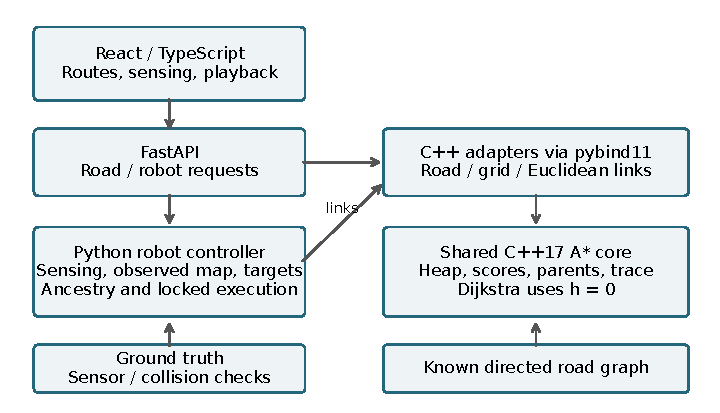
\includegraphics[width=\textwidth]{architecture.pdf}
\caption{Implemented system boundaries. Ground truth enters sensing and motion validation; the continuous planner receives observations and verified links. Traces support frontend playback.}
\label{fig:architecture}
\end{figure}

\source{include/astar/search.hpp} defines generic search, counters, and traces. Problems supply neighbors, heuristic, goal predicate, and state hash/equality. Adapters share this contract without coordinate or equal-cost assumptions. Dijkstra disables the heuristic in the same core.

\subsection{Road Representation and Coordinate Requests}
The OSM-derived graph has 2,986 vertices and 7,152 directed edges, with polyline metadata separate from adjacency (Fig.~\ref{fig:roads}). Coordinate queries scan and project onto road segments using latitude-scaled coordinates. Cumulative Haversine lengths determine fraction $r$; projection is a local approximation.

For directed edge $u\rightarrow v$ of weight $w$, a snapped start connects forward with $(1-r)w$, and a snapped goal connects from $u$ with $rw$. Reverse travel requires a corresponding reversed polyline and uses its own weight and fraction. Two ordered positions on one directed edge obtain a direct connection of $(r_g-r_s)w$ when $r_g\geq r_s$. Endpoints reuse real nodes. Virtual states and partial edges belong only to the request adapter; the base graph is unchanged. Partial route geometry is sliced along the original polyline. The heuristic scale is also reduced if a partial edge requires it. Thus floating-point or geometric approximations do not justify blindly reusing an invalid lower bound.

\begin{figure}[t]
\centering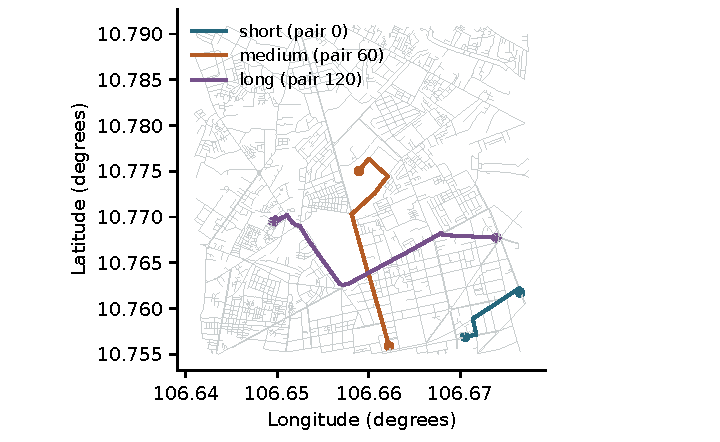
\includegraphics[width=\textwidth]{roads.pdf}
\caption{Representative frozen short, medium, and long road queries. Background is the exported graph, not additional routing information; each highlighted route uses the unchanged C++ adapter. Axes use exported geographic coordinates.}
\label{fig:roads}
\end{figure}

\subsection{Sensing, Exploration, and Observed Ancestry}
Robot Lab supports four or eight directions (diagonal cost 1.5, no corner cutting); grid BAR uses four unit-cost directions. Continuous polygon, seeded maze, and indoor modes retain arbitrary straight-link headings.

The sensor uses 72 uniform directions and rays near visible vertices. First-hit range, blocker margins, and checked free triangles conservatively approximate visibility before union into $F_k$. The sensing disk is not the observed region. Policy receives observations, not hidden polygons/topology; grid evaluation gates are read only after navigation.

Each exploration node records its position, history index, branch ID, parent ID, and remaining candidates. A stack represents active ancestry. Rounded target identities prevent immediate repetition; deferred targets can be reconsidered after map or observation changes. Radar-informed ranking estimates visible frontier opportunity from known boundary segments and discounts travel using direct Euclidean distance. This proxy is not a C++ \astar{} path-cost estimate or a guaranteed observation gain. Low gain alone does not exhaust a branch; uncertain occluded candidates remain eligible through a conservative fallback.

Recovery transfers deferred child alternatives, preserves siblings, and locks execution to the anchor. Graph-blocked and exhausted decisions remain distinct. Playback shows sensing, plans, moves, branches, and returns, with graph debugging hidden by default. Search traces expose $g,h,f$ and parents; continuous frames are higher-level events. Interpolation adds no backend motion.

\section{A* Algorithm Implementation}
\subsection{Queue, Records, and Improved Paths}
An \source{unordered_map} stores best $g$, parent, and last-expanded $g$ per state; a \source{priority_queue} stores state, inserted $g,h,f$, and insertion order. Lexicographic $(f,h,\mathrm{order})$ selects lower $f$, lower $h$, then earlier insertion. Determinism requires deterministic neighbor enumeration.

Algorithm~\ref{alg:core} summarizes the actual implementation. There is no decrease-key operation: an improved path pushes a new entry. An old entry whose stored $g$ exceeds the current record is stale and skipped. An entry no better than the last-expanded value is also skipped. A strictly smaller $g$ is still eligible after prior expansion. This preserves reopening instead of treating CLOSED as a permanent visited flag.

\begin{algorithm}[H]
\caption{Shared C++ search (trace and counters omitted)}\label{alg:core}
\begin{algorithmic}[1]
\Require Problem neighbors, heuristic, goal predicate; start $s$, goal $t$
\State Initialize records with $g=\infty$, no parent or expanded value
\State $g[s]\gets0$; push $(s,0,h(s),h(s),\mathrm{order}{+}{+})$
\While{OPEN is not empty}
  \State Pop minimum entry $e$ with state $u$
  \If{$e.g>g[u]$ or ($u$ expanded and $e.g\geq g_{\rm expanded}[u]$)}
    \State \textbf{continue}
  \EndIf
  \State $g_{\rm expanded}[u]\gets e.g$
  \If{problem goal predicate holds for $u,t$}
    \State \Return predecessor chain reversed, cost $e.g$
  \EndIf
  \For{outgoing $(u,v,w)$}
    \State Validate finite $w\geq0$; $a\gets e.g+w$
    \If{$a<g[v]$}
      \State $g[v]\gets a$; parent$[v]\gets u$
      \State Validate $h(v)$ and finite sum; push $(v,a,h(v),a+h(v),\mathrm{order}{+}{+})$
    \EndIf
  \EndFor
\EndWhile
\State \Return not found, empty path, infinite internal cost
\end{algorithmic}
\end{algorithm}

The engine checks finite nonnegative weights/estimates and rejects overflow; adapters establish admissibility. Relaxation uses strict improvement, with tolerances only in external validation. Reconstruction reverses predecessors from goal to the parentless start. Start equals goal returns a singleton of zero cost; unreachable search returns an empty path, failure, and internal infinity serialized as nullable cost.

For a finite graph, consistent heuristic, binary heap, and expected constant hashing time, lazy entries give a conservative $O((|V|+|E|)\log(|V|+|E|))$ time and $O(|V|+|E|)$ auxiliary-space bound. Geometry and traces add costs. Inconsistent estimates may reopen states, invalidating a single-expansion bound.

\subsection{Application Heuristics and Trace Semantics}
For a road edge, define geographic distance $d_H$. The loader chooses a scale $\alpha\leq1$ respecting $\alpha d_H(u,v)\leq w(u,v)$ and uses $h(u)=\alpha d_H(u,t)$. By the spherical-distance triangle inequality, this implies Eq.~\ref{eq:consistency}. The frozen graph validates every directed edge and retains $\alpha=1$. Directionality does not invalidate the geometric lower bound. Four-direction unit grids use Manhattan distance; the educational eight-direction grid uses $\max(dx,dy)+0.5\min(dx,dy)$ for its actual 1.5 diagonal cost. Euclidean weights in the continuous visibility adapter make Euclidean goal distance consistent by the ordinary triangle inequality.

Expanded nodes count valid pops, including goal and re-expansions; generated nodes count all pushes. Unique counts are separate. Examined and relaxed edges count scanned neighbors and improvements. Trace events expose discovery, updates, expansion, closure, and goal scores. Stale entries are skipped; timing disables traces.

\subsection{Executed Return Certificate}
Let $T=(a=x_0,\ldots,x_m=b)$ be the actual entry trajectory from the selected observed anchor $a$ to current $b$, with length $L_T$. Under static obstacles, sound observed-free checks, and reversible point motion, its reverse is a feasible return of the same length. Recorded waypoints and verified links preserve this candidate. If those links appear in the current planning graph, exact graph-optimal \astar{} gives $L_{A^*}\leq L_T$. The controller additionally checks the proposed route's endpoints, segment coverage, and length before accepting it. If planning fails or the route exceeds the entry bound, it verifies and uses the recorded reverse.

Execution follows the entire accepted return without switching to exploration. The simulator records the executed geometric length $L_R$ and requires
\begin{equation}
L_R\leq L_T+\varepsilon,\qquad
\|x_{\rm end}-a\|_2\leq\varepsilon,
\label{eq:return}
\end{equation}
using the implementation's numerical checks. New sensing during return may add observations, but does not change its destination. Consequently the certificate concerns an observed-anchor episode with reversible verified entry and locked execution. It does not certify arbitrary semantic BAR boundaries, physical disk clearance, universal detection, or complete navigation. A reversed-entry fallback establishes the bound without showing that \astar{} shortened that episode; the trace must distinguish these outcomes.

\section{Experimental Methodology}
\subsection{Frozen Inputs and Controlled Road Comparison}
The baseline is commit \source{04c4846}; manifests pin map, snapshot, and result hashes. The unmodified authors' checkout is verified Git commit \source{8bbbfb8}. The recorded host is Windows 11, Intel Core 7 240H (16 logical processors), and approximately 15.7 GiB RAM. CMake builds C++17 Release with MSYS2 UCRT64 g++; the binding runs in Python 3.12.10 and original ASP in Python 3.14.2. These are different implementation environments. CPU frequency and host load are not controlled; timings are descriptive.

Road selection sampled 6,000 directed candidates with seed 20261009; 5,965 were reachable. Dijkstra distance ranks define three strata at approximately 2,086.98 and 3,273.44 m, retaining 60 queries per stratum. A manifest wording mentions 6,000 reachable distances, but the count and actual selection are 5,965. The frozen selection is unchanged.

Only the heuristic flag differs between methods. One untimed call per method precedes seven alternating-order batches: 20, 10, and 5 calls in the respective strata. Per-pair time is the median batch mean per call. Loading, snapping, HTTP, rendering, and traces are excluded; common timed status/cost checks remain.

\subsection{Source Audit and Shared-State Robot Requests}
The original source computes and logs an ASP but assigns its selected open point as the next coordinate. The coordinate update contains no interpolation along the ASP. The paper's Algorithm 2 specifies movement along DAP. An independent audit finds four hypothetical straight chords crossing interiors in a dead-end reproduction and one in a bugtrap reproduction, while planned ASP segments avoid obstacle interiors. Since coordinate transitions alone do not establish a continuous physical trajectory, the 48-configuration end-to-end matrix remains unexecuted as a comparable motion experiment. We do not report its blocked cells as failures or compare its coordinate-chord distance with our executed travel.

Frozen requests preserve position, target, original sights, skeleton, ASP, and provenance. The original routine is replayed unchanged. Our A* uses scan centers and identical endpoints, with analytic whole-segment certification in recorded sights. This adapter preserves circular boundaries rather than the application's polygon approximation. Full polygons enter only post-plan validation.

Eligibility requires more than two skeleton vertices, before local outcomes. Three cohorts contain 43, 75, and 233 decisions. Prospective selection preceded ten episodes at radii 10/20/30, capped at 60 iterations; capped outcomes remain. Decisions are correlated, and prior held-out bugtrap geometry overlaps earlier states.

\begin{table}[t]
\caption{Frozen robot decision accounting. Direct exclusions do not invoke bundle refinement; they are retained in the raw audit.}\label{tab:eligibility}
\centering\begin{tabular}{lrrr}\toprule
Cohort & Captured & Eligible & Excluded\\\midrule
Initial &43&6&37\\
Prior held-out &75&1&74\\
Prospective extension &233&14&219\\\midrule
Combined &351&21&330\\\bottomrule
\end{tabular}
\end{table}

Direct exclusions comprise 176 source-visible and 154 strict-range-boundary cases. Boundary convention explains endpoint predicate differences, with no missing-input or eligibility-checker mismatch. All 21 eligible requests remain, regardless of planner outcome.

\subsection{Validity, Metrics, and Timing Boundaries}
Primary robot validity requires matching endpoints within $10^{-7}$, full observed-sight segment coverage, and no polygon-interior entry; boundary contact is permitted. Strict point validity rejects boundary contacts as well. Radius-0.5 clearance is a separate offline diagnostic, not the planned collision model. Event-based segment certification uses tolerance $10^{-9}$; sampled predicate comparisons supplement it rather than prove universal sensor equivalence. Across all cohorts, 175,500 membership samples and 111,672 graph-link samples have no unexplained mismatch or uncovered sample. All 865 recorded ASP segments are sight-certified; 1,128 accepted A* graph links avoid polygon interiors and boundaries offline.

Length is a sum of Euclidean polyline segments. An all-turn count uses wrapped heading changes exceeding $10^{-6}$ radians; an interpretable significant-turn count uses changes greater than $15^\circ$. Neither is a motor command count. ASP critical-line counts and A* expansions are not interchangeable operations. Robot component timing uses three warm-ups and 31 measured calls per state, then medians across state medians. ASP core excludes source skeleton generation; A* graph construction includes observed-link certification and is separated from its binding/search call. Medians of components need not sum to a median pipeline time.

Supporting experiments retain 20 legacy versus radar pairs, 20 full versus cached frontier pairs, 12 sensor episodes, and an indoor parent trace. They evaluate our simulator separately. Statistics are paired by configuration before aggregation; no significance or population-superiority claim follows. Report scripts read frozen results without overwriting them.

\section{Results and Discussion}
\subsection{Road Cost Agreement and Search Effort}
All 180 matched road queries return equal costs under A*, Dijkstra, and the frozen offline reference within $10^{-6}$ m. The graph validator reports zero heuristic edge violations and scale 1.0. Separately retained edge cases cover start equals goal, unreachable targets, directionality, and edge-midpoint snapping. These checks support correctness on the tested graph; agreement alone is not a proof for every possible adapter.

\begin{table}[H]
\caption{Frozen road results; 60 pairs per stratum. Expansion and time columns are marginal medians; reduction and ratio are medians of paired statistics.}\label{tab:road}
\centering\begin{tabular}{lrrrr}\toprule
Stratum & Expanded A*/D & Reduction & Time A*/D ($\mu$s) & Ratio\\\midrule
Short &101 / 505&78.6\%&44.95 / 128.09&0.324\\
Medium &301 / 1,592&77.4\%&282.95 / 1,117.24&0.287\\
Long &714.5 / 2,588.5&68.6\%&771.46 / 1,883.19&0.449\\\bottomrule
\end{tabular}
\end{table}

\begin{figure}[t]
\centering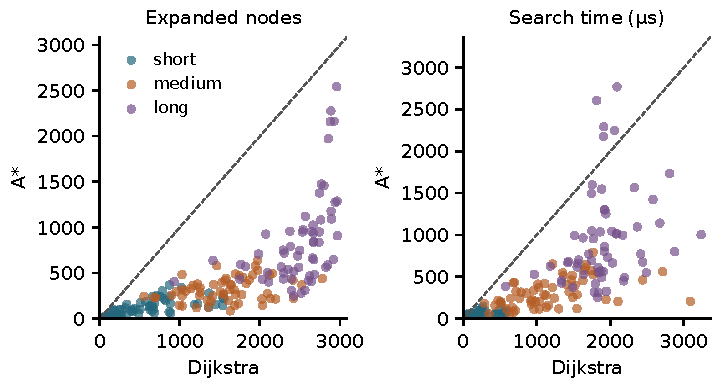
\includegraphics[width=\textwidth]{road-effort.pdf}
\caption{Matched road search effort and search-call timing. Points below the diagonal favor A*. Each stratum has 60 queries; all 180 costs agree. Timing excludes graph loading, snapping, API, and rendering.}
\label{fig:road-effort}
\end{figure}

Table~\ref{tab:road} and Fig.~\ref{fig:road-effort} show fewer expansions in every A* run, with median paired reduction 76.0\%. A* is faster in 173 cases, Dijkstra in seven; the median time ratio is 0.338, range 0.061--1.435, with pair 167 the largest regression. The heuristic improves descriptive effort and time on this network without winning every timing pair. Paired ratios are not ratios of marginal medians. This known-graph comparison controls representation more tightly than the robot study.

\subsection{Robot Local Geometry and Path Length}
Both local planners find paths for all 21 eligible requests, with correct endpoints and primary interior-only validity in all 21. These are local planning successes, not 21 successful autonomous missions. Of the ten prospective source episodes, nine reach the goal and one reaches its iteration cap; its eligible states remain. Figure~\ref{fig:observed} shows an observed-space request and the two returned paths. No hidden polygons are supplied to either local planner.

\begin{figure}[t]
\centering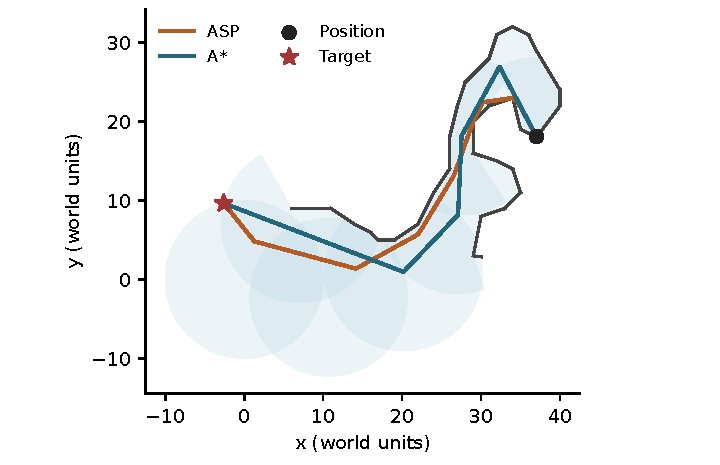
\includegraphics[width=\textwidth]{robot-observed.pdf}
\caption{Representative frozen dead-end request. Visible blocker fragments and approximate display sight footprints show recorded knowledge; ASP and scan-center A* use the same position and target. Sight footprints are display approximations; benchmark link admission uses analytic whole-segment certification. Hidden obstacles are omitted.}
\label{fig:observed}
\end{figure}

\begin{table}[H]
\caption{Local robot outcomes by cohort. ``Shorter'' counts follow the primary point convention. Two prospective cases have equal lengths. Delta is the median paired A* minus ASP length in world units.}\label{tab:robot}
\centering\begin{tabular}{lrrrr}\toprule
Cohort &Pairs&ASP shorter&A* shorter&Delta\\\midrule
Initial &6&5&1&$+7.403$\\
Prior held-out &1&1&0&$+1.654$\\
Prospective &14&3&9&$-2.492$\\\midrule
Combined &21&9&10&$0.000$\\\bottomrule
\end{tabular}
\end{table}

ASP is shorter in nine requests, A* in ten, and two are equal. The paired delta median is zero, mean $+2.981$, range $[-10.707,+44.266]$ world units. Cohort composition matters: five of six initial cases favor ASP, nine of fourteen prospective cases favor A*. One held-out eligible request cannot establish generalization. Figure~\ref{fig:robot-length} retains all pairs.

\begin{figure}[t]
\centering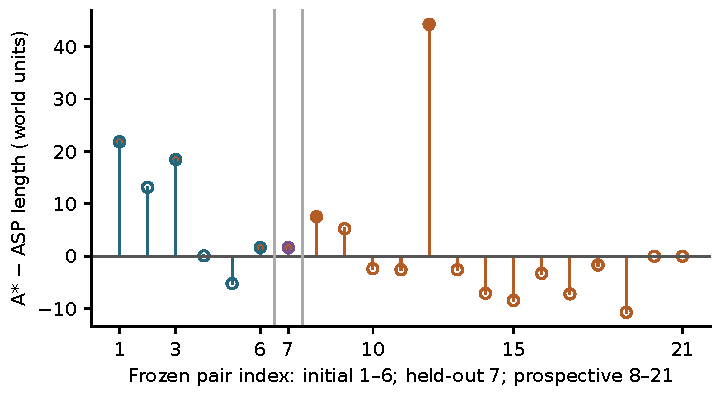
\includegraphics[width=\textwidth]{robot-length.pdf}
\caption{All 21 eligible local requests, grouped by frozen cohort. Positive A* minus ASP differences favor ASP. Filled orange markers indicate ASP boundary contact under the strict convention; these paths remain primary interior-valid.}
\label{fig:robot-length}
\end{figure}

Strict no-contact validity differs: ASP passes 15 of 21, and A* passes 21 of 21. All six boundary-touching ASP paths are shorter under the permissive point convention. In the largest difference, \source{P02-_map_deadend-01}, ASP is 15.734 units versus A* 60.000, but ASP touches a boundary. Among the 15 jointly strict-valid pairs, ASP is shorter in three, A* in ten, and two are equal; the median paired difference is $-2.584$. This secondary analysis changes the feasible interpretation and must not replace the prespecified primary result. It illustrates how strict links through sparse centers and geometric refinement produce different paths.

Radius-0.5 clearance passes only nine ASP and eleven A* paths, precluding disk-safety claims. Significant-turn medians are two and one respectively; paired all-turn delta median is $-2$. Tiny ASP bends can inflate all-turn counts without corresponding physical steering. ASP vertices can lie inside bundles absent from the sparse A* graph, so mixed lengths do not contradict graph-optimal search.

\begin{figure}[t]
\centering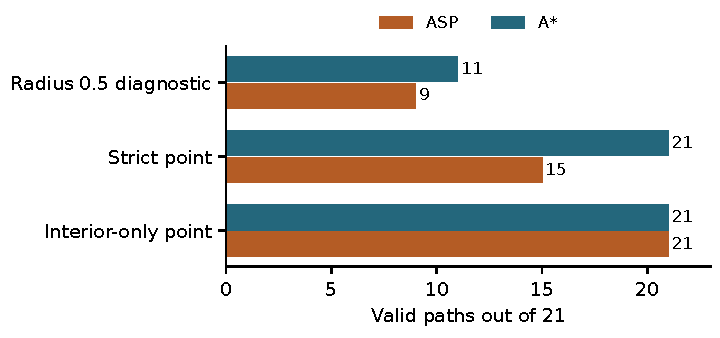
\includegraphics[width=\textwidth]{robot-validity.pdf}
\caption{Validity outcomes for the same 21 requests. Primary point validity allows boundary tangency; strict validity forbids it. Disk clearance is only a post-plan sensitivity check, not a guarantee of executed finite-robot motion.}
\label{fig:validity}
\end{figure}

\subsection{Robot Computation Components}
Figure~\ref{fig:runtime} separates the measured components. Across state medians, ASP core time is 62.655 ms, critical-line construction 0.319 ms, and optimization 62.400 ms. A* link-build time is 42.102 ms, binding/search 0.0263 ms, and the median per-state build-plus-call sum 42.142 ms. The small C++ call is a search on already constructed sparse graphs, while Python geometric certification can dominate its surrounding pipeline.

\begin{figure}[t]
\centering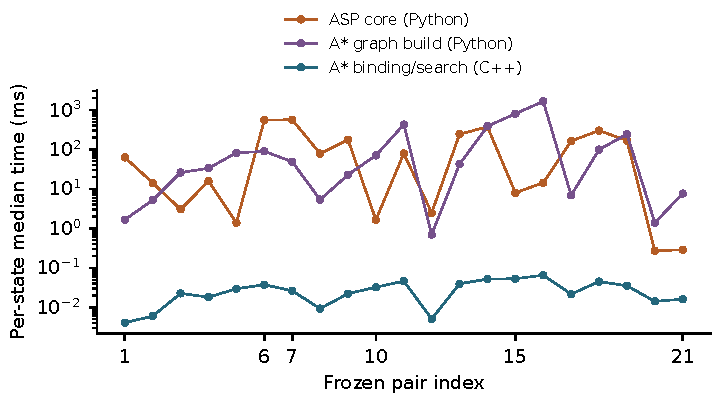
\includegraphics[width=\textwidth]{robot-runtime.pdf}
\caption{Per-state median local computation times (three warm-ups, 31 calls). A logarithmic axis exposes component scale. ASP core excludes skeleton generation; A* build includes observed-link certification. Components and languages differ, so isolated search ratios are not algorithm-only speedups.}
\label{fig:runtime}
\end{figure}

Dividing ASP core time by the C++ call would misrepresent differing languages and preparation. Even build-plus-call and ASP core omit different upstream work. The justified conclusion is that construction matters and C++ search is small for these requests, not that an intrinsic algorithm speedup was established.

\subsection{Supporting Online Behavior and Recovery}
The legacy and radar policies both reach the goal in 20 paired episodes. Radar travels less in 18 and more in two, with median paired delta $-95.419$ world units. Its largest regression is $+70.772$ in Complex Irregular Labyrinth at radius 7. This supports retaining radar ranking as a useful non-dominating policy. It does not prove an optimal exploration order or justify exhausting low-score frontiers. Twelve sensor-radius episodes all reach their goals, but the radius-5 and radius-7 distance medians are 92.909 and 113.278 units; greater range does not monotonically shorten travel in this sample.

Cached and full frontier construction preserve complete playback, recovery outcomes, status, and distance in all 20 pairs. Their median frontier-processing times are 639.166 and 46.723 ms respectively. These are accumulated component times per episode, not end-to-end timings. Cache validity depends on invalidation when newly observed free geometry or walls change the frontier mask. The paired equivalence is concrete evidence for the tested indoor and maze configurations, not a universal assertion about arbitrary geometric updates.

\begin{figure}[t]
\centering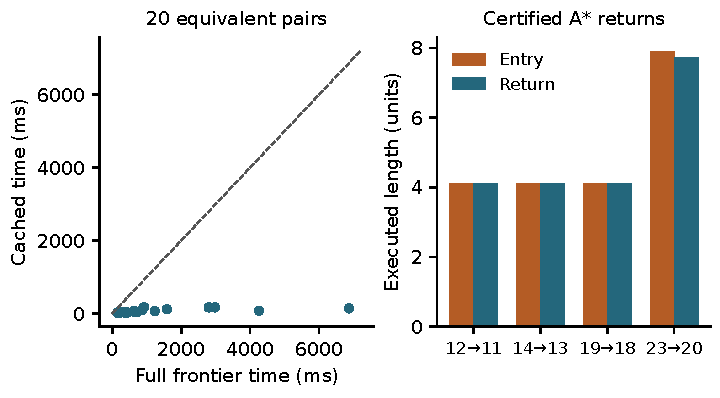
\includegraphics[width=\textwidth]{supporting.pdf}
\caption{Supporting evidence from our online simulator. Left: paired frontier processing with equivalent playback in 20 cases. Right: four observed indoor branch returns, each certified and marked nonfallback in the frozen trace. These are separate from the local authors-versus-A* comparison.}
\label{fig:support}
\end{figure}

Four certified nonfallback indoor returns demonstrate genuine C++ A* recovery. Verified reverse-entry fallback is distinct. Certification concerns executed length to an observed ancestor; successful unlabelled exits, unreachable fixtures, and budget termination require separate labels. Continuous no-frontier status establishes candidate exhaustion, not unknown-world unreachability.

\section{Limitations and Threats to Validity}
\paragraph{Model validity.} Static obstacles, ideal localization, reversible point motion, and reliable observations exclude probabilistic sensing, pose drift, dynamics, and footprint-aware configuration space. Sampled sensing may miss narrow occluded regions; accumulated free space differs from the sensing disk. Finite frontier candidates and budgets preclude inferring completeness in arbitrary polygonal worlds from fixture success.

\paragraph{Scope of guarantees.} Missing geometric vertices can make graph-optimal paths longer than continuous optima. The return bound requires verified reversible entry, appropriate endpoints, and locked execution; it proves neither universal BAR identification nor optimal online travel. The paper's approximation and restricted convergence arguments do not transfer to this controller. Our BAR-inspired application retains the stated restrictions rather than reproducing all published mechanisms.

\paragraph{Comparison validity.} Shared observations do not imply shared graphs. Permissive and strict boundaries change interpretation; point validity does not establish disk safety. Source transitions and ASPs do not expose compatible continuous execution, keeping end-to-end comparison gated. Our adapter differs from the paper's grid baseline, so this is not reproduction of its numerical tables. Local timings and selected examples cannot establish superiority.

\paragraph{Sampling and timing.} One road network, convenience robot maps, correlated decisions, overlapping held-out geometry, and 21 eligible requests limit external validity. Prospective selection reduces outcome bias without creating independent random trials. Scheduling, Python versions, compiler settings, batch averaging, and unmatched computation boundaries affect timing. Repetitions and ranges improve auditability without eliminating confounders; paired descriptive results support neither significance claims nor transferable speedup guarantees.

\paragraph{Reproducibility.} Frozen records report four C++ suites, 169 Python tests, 34 frontend tests, and build/lint success, without proving optimal exploration. Report validation checks hashes and statistics without changing results. Author and affiliation remain unverified configurable metadata.

\section{Conclusion and Future Work}
The project implements a reusable C++17 A* engine and two distinct applications. Road Navigation is a known directed shortest-path problem with a verified geographic lower bound. Blind-Alley Robot Navigation combines limited observations, conservative geometric links, exploration decisions, repeated A*, and locked observed-parent returns. The latter uses A* centrally while preserving the distinction between search, exploration, and execution.

The frozen road study establishes cost agreement on all 180 queries and substantial descriptive reductions in search effort. The robot study provides a defensible shared-state comparison: 21 retained nontrivial requests, both planners primary-valid in all, mixed length outcomes, and explicit boundary and component-timing caveats. Supporting runs demonstrate practical frontier-cache savings with unchanged tested playback and genuine A*-computed certified returns. They also retain exploration regressions and nonmonotonic sensing results.

For a university algorithms demonstration, the defensible claim is an implemented and reproducibly evaluated system with graph-level correctness assumptions and conditional recovery guarantees. Future investigation could test independent maps, verified footprint-aware geometry, sensing approximation error, and matched planning pipelines. Incremental replanning or richer geometric vertices would require new controlled experiments.

\bibliographystyle{splncs04}
\bibliography{references}
\end{document}
